\chapter{Planificación}

\section{Fases y entregas}

\subsection{Fases}

Como este va a ser un proyecto que ya cuenta con un trabajo previo realizado, la fase inicial de gestión va a ser muy breve porque se parte de que ya se han realizado varias reuniones y el proyecto está parcialmente funcionando, por lo que no se parte de cero, es una ampliación de un proyecto inicial.

\begin{itemize}
  \item \textbf{Fase 1:} Especificaciones del proyecto
  \item \textbf{Fase 2:} Planificación
  \item \textbf{Fase 3:} Análisis y diseño
  \item \textbf{Fase 4:} Implementación
  \item \textbf{Fase 5:} Pruebas
  \item \textbf{Fase 6:} Documentación
\end{itemize}

\subsection{Lista de entregas}

Se harán una serie de breves informes sobre el contenido de cada una de las fases de planificación del proyecto.

\begin{itemize}
  \item \textbf{Fase 1:} Especificación del proyecto.
  \begin{itemize}
    \item Descripción: Se establecen los objetivos a cumplir para que el desarrollo del proyecto se considere completado.
    \item Tipo: informe.
  \end{itemize}
  \newpage
  \item \textbf{Fase 2:} Planificación.
  \begin{itemize}
    \item Descripción: Se desarrolla la documentación con toda la planificación del desarrollo del proyecto.
    \item Tipo: informe.
  \end{itemize}
  \item \textbf{Fase 3:} Análisis y diseño.
  \begin{itemize}
    \item Descripción: Todos los aspectos del proyectos son analizados para concretar la forma de desarrollarlo.
    \item Tipo: informe.
  \end{itemize}
  \item \textbf{Fase 4:} Implementación.
  \begin{itemize}
    \item Descripción: Con el proyecto ya planificado y diseña se pasa programar todo lo necesario para cumplir los objetivos.
    \item Tipo: software.
  \end{itemize}
  \item \textbf{Fase 5:} Pruebas.
  \begin{itemize}
    \item Descripción: Una vez este todo programado, se pasa a validar con diferentes procedimientos que el proyecto funciona correctamente tomando como referentes unas métricas propias.
    \item Tipo: informe y software.
  \end{itemize}
  \item \textbf{Fase 6:} Documentación.
  \begin{itemize}
    \item Descripción: Para finalizar el proyecto se realiza toda la documentación informativa y explicativa.
    \item Tipo: informe.
  \end{itemize}
\end{itemize}

\section{Estructura de descomposición del trabajo}

El diagrama de estructura de descomposición del trabajo (figura 3.1) es una descomposición jerárquica de las diferentes fases y entregas en las que está planificado el proyecto.

\newpage
\section{Lista de actividades}

Las actividades que se vayan a desarrollar en cada una de las fases para cada una de las entregas se va a listar junto con una estimación del tiempo que deberían tomar en ser cumplidas.

\begin{itemize}
   \item \textbf{Especificaciones del proyecto:}
   \begin{itemize}
    \item Determinación de objetivos.
    \item Determinación de requisitos.
    \item \underline{\textit{Estimación: 9 horas}}
    \end{itemize}
\end{itemize}

\begin{itemize}
   \item \textbf{Planificación:}
   \begin{itemize}
    \item Lista de actividades.
    \item Recursos humanos.
    \item Presupuesto.
    \item Temporización.
    \item \underline{\textit{Estimación: 18 horas}}
   \end{itemize}
\end{itemize}

\begin{itemize}
   \item \textbf{Análisis y diseño:}
   \begin{itemize}
    \item Análisis de requisitos.
    \item Diagramas.
    \item Metodología de desarrollo.
    \item Descripción estructural.
    \item \underline{\textit{Estimación: 36 horas}}
   \end{itemize}
\end{itemize}

\begin{itemize}
 \item \textbf{Implementación:}
 \begin{itemize}
  \item Herramientas seleccionadas.
  \item Solucionar problema de generación de páginas.
  \item Implementar tests unitarios.
  \item Implementar test de cobertura.
  \item Introducir integración continua.
  \item Agregar despliegue automático.
  \item Actualizar aprovisionamiento.
  \item \underline{\textit{Estimación: 90 horas}}
 \end{itemize}
\end{itemize}

\newpage
\begin{itemize}
 \item \textbf{Pruebas:}
 \begin{itemize}
  \item Pruebas de software.
  \item Pruebas de carga.
  \item \underline{\textit{Estimación: 30 horas}}
 \end{itemize}
\end{itemize}

\begin{itemize}
 \item \textbf{Documentación:}
 \begin{itemize}
  \item Documentación de la aplicación.
  \item Manual de usuario.
  \item Documentación del proyecto.
  \item \underline{\textit{Estimación: 30 horas}}
 \end{itemize}
\end{itemize}

\section{Recursos humanos}

Como este es un proyecto que comenzó su desarrollo en la Oficina de Software Libre de la Universidad de Granada, cuento con el apoyo de todos sus colaboradores, además del resto de becarios que se encuentran realizando prácticas en empresa en ella como es mi situación actual, además, siendo el tutor de este proyecto el director de la propia oficina.

\section{Presupuesto}

Una de las ventajas de usar software libre es que no es necesario adquirir licencias por las que haya que pagar para realizar su uso, como todas las herramientas que usen (al igual que las que se generen) serán software libre, el coste en software para el desarrollo será cero.

\bigskip

El único recurso necesario es el servidor en que estará instalada el portal, servidor ya que adquirido anteriormente, por lo que tampoco es necesario considerarlo un gasto a afrontar de cara al desarrollo.

\section{Temporización}

Para percibir de forma más visual la planificación temporal de las tareas se incluyen la figura 3.2 con una tabla indicando los plazos de cada tarea y la figura 3.3 con un diagrama de Gantt de dichas tareas.
\newpage

\begin{figure}[!ht]
  \begin{center}
    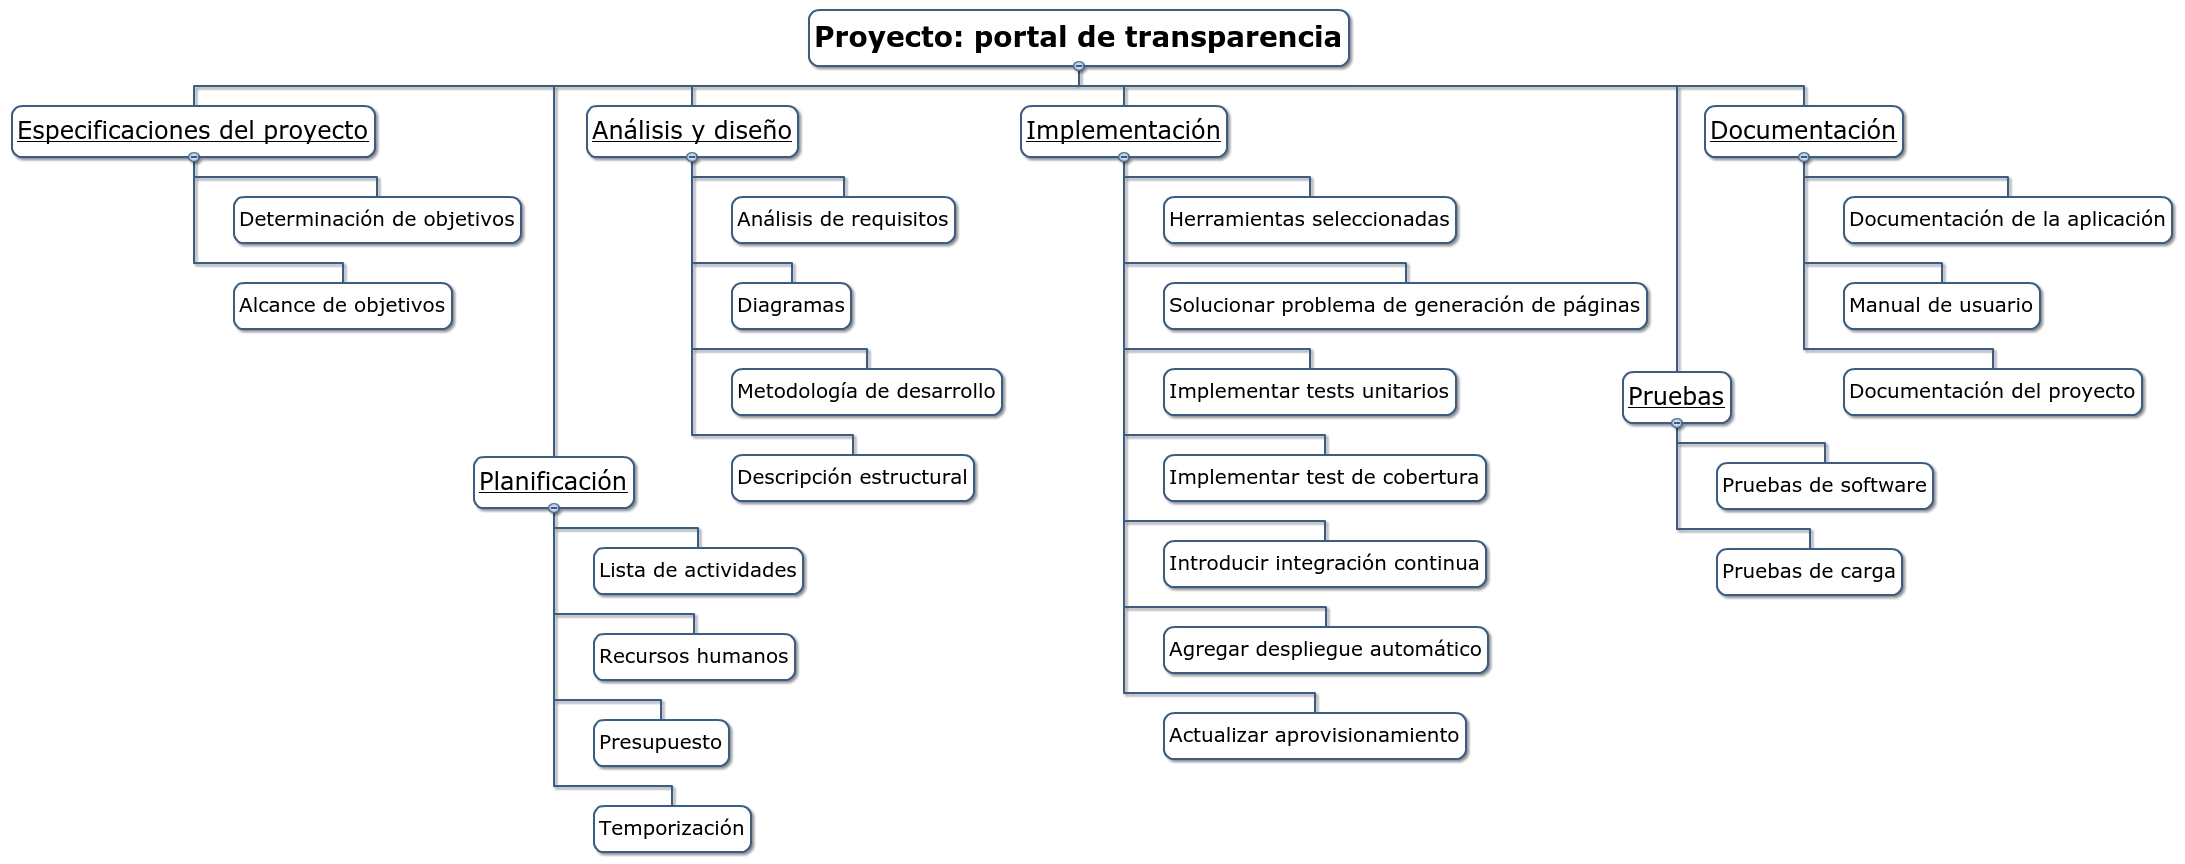
\includegraphics[scale=0.25,angle=90]{imagenes/diagrama_edt.png}
    \caption{Diagrama de estructura de descomposición de trabajo}
    \label{fig:diag_edt}
  \end{center}
\end{figure}

\newpage
\begin{figure}[!ht]
  \begin{center}
    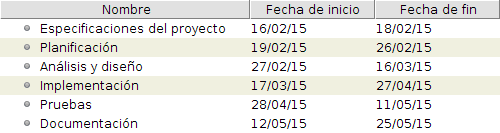
\includegraphics[width=1\textwidth]{imagenes/tempo_tareas.png}
    \caption{Temporización de las tareas}
    \label{fig:tempo_tareas}
  \end{center}
\end{figure}

% \begin{table}[!ht]
%   \begin{center}
%     \begin{tabular}{|l|l|l|}
%       \hline
%       \multicolumn{1}{|c|}{{\bf Nombre}} & \multicolumn{1}{c|}{{\bf Fecha de inicio}} & \multicolumn{1}{c|}{{\bf Fecha de fin}} \\ \hline
%       Especificaciones del proyecto      & 16/02/15                                   & 18/02/15                                \\ \hline
%       Planificación                      & 19/02/15                                   & 26/02/15                                \\ \hline
%       Análisis y diseño                  & 27/02/15                                   & 16/03/15                                \\ \hline
%       Implementación                     & 17/03/15                                   & 27/04/15                                \\ \hline
%       Pruebas                            & 28/04/15                                   & 11/05/15                                \\ \hline
%       Documentación                      & 12/05/15                                   & 25/05/15                                \\ \hline
%     \end{tabular}
%     \caption{Temporización de las tareas}
%     \label{table:tempo_tareas}
%   \end{center}
% \end{table}

\begin{figure}[!ht]
  \begin{center}
    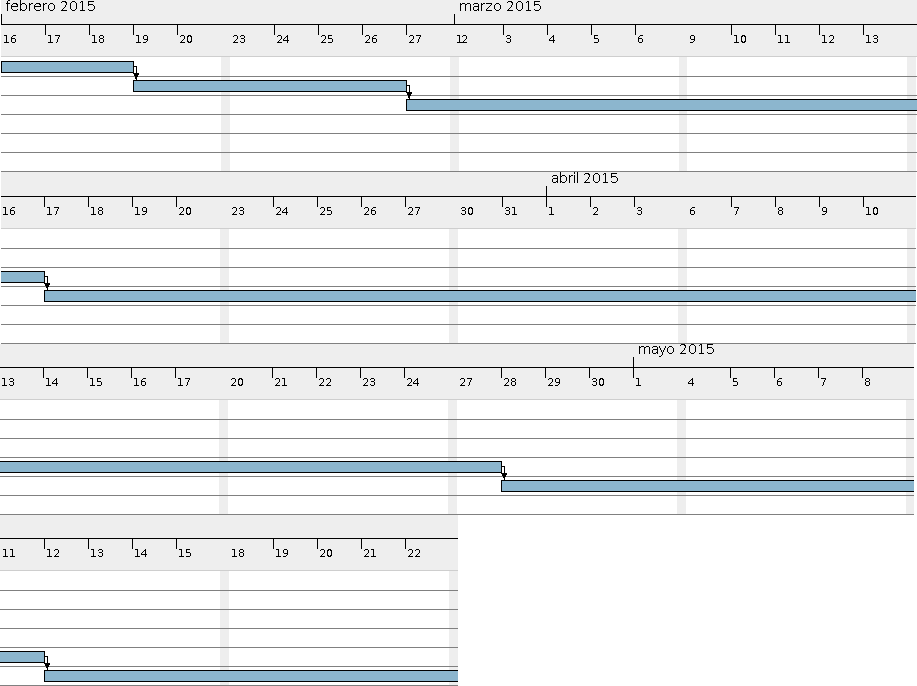
\includegraphics[width=1\textwidth]{imagenes/diagrama_gantt.png}
    \caption{Diagrama de Gantt}
    \label{fig:diag_edt}
  \end{center}
\end{figure}